\documentclass[12pt]{article}
% controlling the geometry of the page:
\usepackage[margin=1in, paperwidth=8.5in, paperheight=11in, landscape]{geometry} 
\usepackage{amsmath, amssymb} % useful math symbols and environments

\usepackage{multicol} % multiple columns side-by-side

\usepackage{amsthm} % Theorem-like environments
\theoremstyle{definition} % Without this line, theorem statements (and therefore problem statements etc.) show up in italic text.
\newtheorem{conjecture}{Conjecture}
\newtheorem{problem}{Problem}
\newtheorem*{remark}{Remark}
\newtheorem*{definition}{Definition}

% pretty colors!
\usepackage[dvipsnames]{xcolor}
\colorlet{darkgrey}{black!70}
\colorlet{darkgreen}{green!50!black}


\usepackage{tikz} % for drawing diagrams
\usetikzlibrary{arrows,automata,positioning} 
\usetikzlibrary{decorations.markings}
\usetikzlibrary{decorations.pathreplacing}
\usetikzlibrary{patterns}
\usetikzlibrary{shapes.geometric}

\usepackage{visualalgebra}
\usepackage{graphicx} % for inserting figures with \includegraphics
\usepackage{setspace} % for controlling space between lines, paragraphs, etc.

\usepackage{fancyhdr} % for controlling headers and footers
\usepackage{newtx} % changes the default font family
\usepackage[shortlabels]{enumitem} % controllable labels for ordered and unordered lists

\usepackage{hyperref} % controls hyperlinks, both internal and external
\hypersetup{
    colorlinks=true,
    urlcolor=blue,
}

\setlength{\headheight}{14.5pt}

% I don't like how LaTeX renders section headings by default
\renewcommand{\section}[1]{\begin{center} \textbf{#1} \\\end{center}}
%
\setlength{\parindent}{0in}
%\oddsidemargin=-.25in
\allowdisplaybreaks
\pagestyle{fancy}
\renewcommand{\headrulewidth}{0pt}
\lhead{MATH 312}
\rhead{Spring 2025}
\chead{\textbf{Subgroup lattice of $A_5$}}
%\lfoot{\copyright\ CLEAR Calculus 2010}
\cfoot{}
\renewcommand{\thefootnote}{*} 
\hyphenpenalty=10000 % LaTeX by default really likes hyphenating things

%##################################################################
\begin{document}

\[
  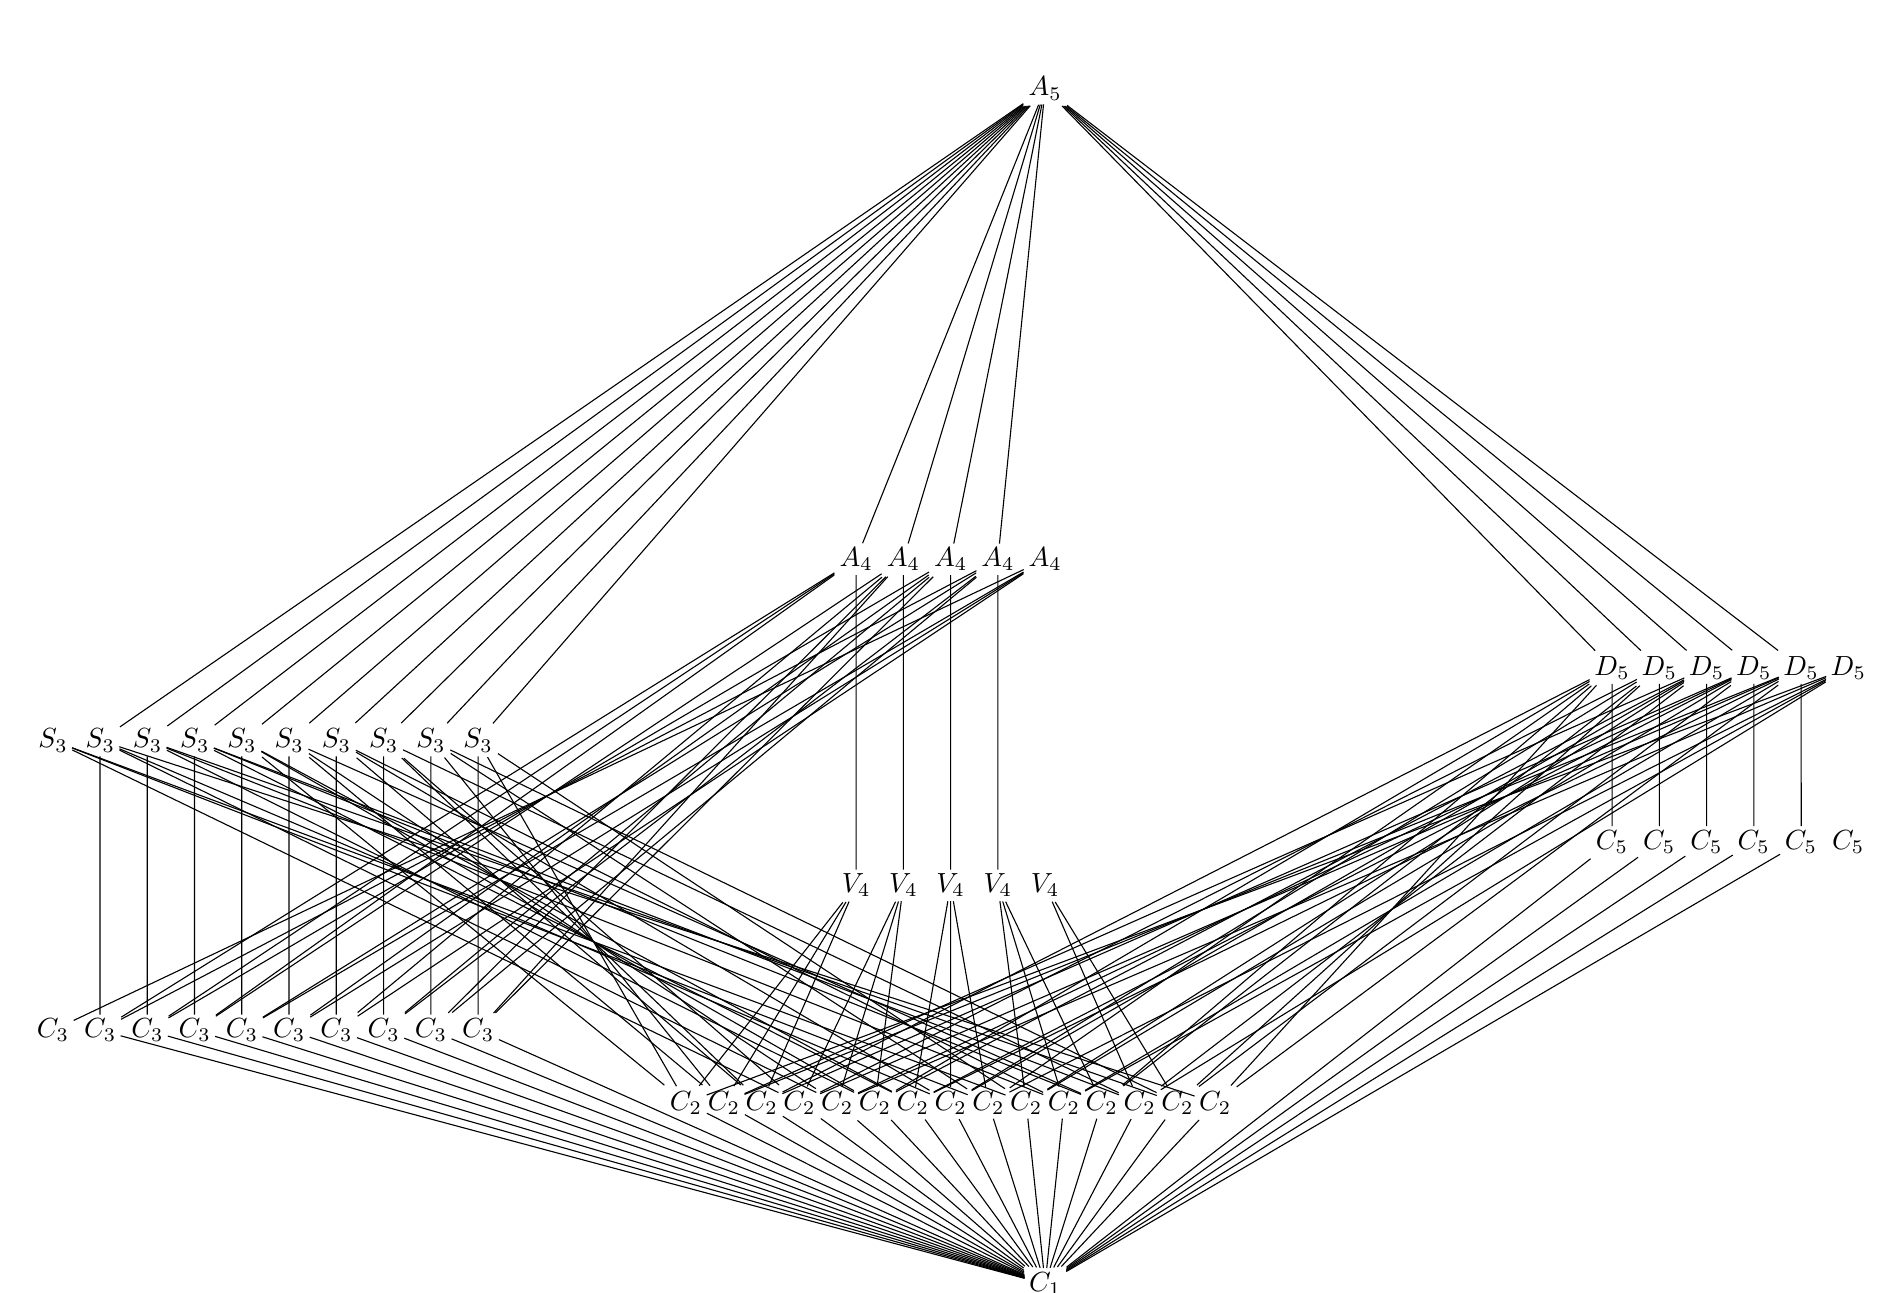
\begin{tikzpicture}[shorten >= -2pt, shorten <= -2pt,yscale=0.92, xscale=1.2]
    \newcommand\Hh{16} % height of A_5
    \newcommand\Hg{9.5} % height of A_4
    \newcommand\Hf{8} % height of D_10
    \newcommand\He{7} % height of S_3
    \newcommand\Hd{5.6} % height of C_5
    \newcommand\Hc{5} % height of V_4
    \newcommand\Hb{3} % height of C_3
    \newcommand\Ha{2} % height of C_2  
    \tikzstyle{R} = [draw]
    \tikzstyle{B} = [draw]
    \tikzstyle{G} = [draw]
    \tikzstyle{O} = [draw]
    \tikzstyle{P} = [draw]
    %%
    \node (A5) at (0,\Hh) {$A_5$};
    \node (12-1)at(-2,\Hg) { $A_4$};
    \node (12-2)at(-1.5,\Hg){ $A_4$};
    \node (12-3)at(-1,\Hg) { $A_4$};
    \node (12-4)at(-.5,\Hg) { $A_4$};
    \node (12-5)at(0,\Hg) { $A_4$};
    %%
    \node (10-1)at(6,\Hf) { $D_5$}; \node (10-2)at(6.5,\Hf) { $D_5$};
    \node (10-3)at(7,\Hf) { $D_5$}; \node (10-4)at(7.5,\Hf) { $D_5$};
    \node (10-5)at(8,\Hf) { $D_5$}; \node (10-6)at(8.5,\Hf) { $D_5$};
    %%
    \node (6-1)at(-10.5,\He){ $S_3$}; \node (6-2)at(-10,\He){ $S_3$};
    \node (6-3)at(-9.5,\He){ $S_3$}; \node (6-4)at(-9,\He) { $S_3$};
    \node (6-5)at(-8.5,\He){ $S_3$}; \node (6-6)at(-8,\He) { $S_3$};
    \node (6-7)at(-7.5,\He) { $S_3$}; \node (6-8)at(-7,\He) { $S_3$};
    \node (6-9)at(-6.5,\He) { $S_3$}; \node (6-10)at(-6,\He) { $S_3$};
    %%
    \node (5-1)at(6,\Hd) { $C_5$}; \node (5-2)at(6.5,\Hd) { $C_5$};
    \node (5-3)at(7,\Hd) { $C_5$}; \node (5-4)at(7.5,\Hd) { $C_5$};
    \node (5-5)at(8,\Hd) { $C_5$}; \node (5-6)at(8.5,\Hd) { $C_5$};
    %%
    \node (4-1)at(-2,\Hc) { $V_4$};
    \node (4-2)at(-1.5,\Hc) { $V_4$};
    \node (4-3)at(-1,\Hc) { $V_4$};
    \node (4-4)at(-.5,\Hc) { $V_4$};
    \node (4-5)at(0,\Hc) { $V_4$};
    %%
    \node (3-1)at(-10.5,\Hb) { $C_3$}; \node (3-2)at(-10,\Hb){ $C_3$};
    \node (3-3)at(-9.5,\Hb) { $C_3$}; \node (3-4)at(-9,\Hb) { $C_3$};
    \node (3-5)at(-8.5,\Hb) { $C_3$}; \node (3-6)at(-8,\Hb) { $C_3$};
    \node (3-7)at(-7.5,\Hb) { $C_3$}; \node (3-8)at(-7,\Hb) { $C_3$};
    \node (3-9)at(-6.5,\Hb) { $C_3$}; \node (3-10)at(-6,\Hb) { $C_3$};
    %%  
    \node (2-1)at(-3.8,\Ha) { $C_2$};
    \node (2-2)at(-3.4,2) { $C_2$};
    \node (2-3)at(-3,\Ha) { $C_2$};
    \node (2-4)at(-2.6,\Ha){ $C_2$};
    \node (2-5)at(-2.2,\Ha) { $C_2$};
    \node (2-6)at(-1.8,\Ha){ $C_2$};
    \node (2-7)at(-1.4,\Ha) { $C_2$};
    \node (2-8)at(-1,\Ha) { $C_2$};
    \node (2-9)at(-.6,\Ha) { $C_2$};
    \node (2-10)at(-.2,\Ha) { $C_2$};
    \node (2-11)at(.2,\Ha) { $C_2$};
    \node (2-12)at(.6,\Ha){ $C_2$};
    \node (2-13)at(1,\Ha) { $C_2$};
    \node (2-14)at(1.4,\Ha) { $C_2$};
    \node (2-15)at(1.8,\Ha) { $C_2$}; 
    %%  
    \node (e)at(0,-.5) { $C_1$};
    %%
    \draw[R] (2-1) to (e); \draw[R] (2-2) to (e); \draw[R] (2-3) to (e);
    \draw[B] (2-4) to (e); \draw[B] (2-5) to (e); \draw[B] (2-6) to (e);
    \draw[G] (2-7) to (e); \draw[G] (2-8) to (e); \draw[G] (2-9) to (e);
    \draw[O] (2-10) to (e); \draw[O] (2-11) to (e); \draw[O] (2-12) to (e);
    \draw[P] (2-13) to (e); \draw[P] (2-14) to (e); \draw[P] (2-15) to (e);
    %%
    \draw (3-2) to (e); \draw (3-3) to (e);
    \draw (3-4) to (e); \draw (3-5) to (e); \draw (3-6) to (e);
    \draw (3-7) to (e); \draw (3-8) to (e); \draw (3-9) to (e);
    \draw (3-10) to (e); 
    %%
    \draw (5-1) -- (e); \draw (5-2) to (e); \draw (5-3) to (e);
    \draw (5-4) to (e); \draw (5-5) to (e);
    %%
    \draw (5-1) -- (10-1); \draw (5-2) to (10-2); \draw (5-3) to (10-3);
    \draw (5-4) to (10-4); \draw (5-5) to (10-5);
    %%
    \draw (6-2) to (3-2); \draw (6-3) to (3-3);
    \draw (6-4) to (3-4); \draw (6-5) to (3-5); \draw (6-6) to (3-6);
    \draw (6-7) to (3-7); \draw (6-8) to (3-8); \draw (6-9) to (3-9);
    \draw (6-10) to (3-10);
    %%
    \draw[R] (A5) to (12-1); \draw[B] (A5) to (12-2); \draw[G] (A5) to (12-3);
    \draw[O] (A5) to (12-4);
    \draw (A5) to (10-1); \draw (A5) to (10-2); \draw (A5) to (10-3);
    \draw (A5) to (10-4); \draw (A5) to (10-5);
    \draw (A5) to (6-2); \draw (A5) to (6-3);
    \draw (A5) to (6-4); \draw (A5) to (6-5); \draw (A5) to (6-6);
    \draw (A5) to (6-7); \draw (A5) to (6-8); \draw (A5) to (6-9);
    \draw (A5) to (6-10); 
    %%
    \draw (2-1) -- (10-6);
    \draw (2-2) -- (10-3); \draw (2-2) -- (10-5);
    \draw (2-3) -- (10-1); \draw (2-3) -- (10-4);
    \draw (2-4) -- (10-2); \draw (2-4) -- (10-5);
    \draw (2-5) -- (10-4); \draw (2-5) -- (10-6);
    \draw (2-6) -- (10-1); \draw (2-6) -- (10-3);
    \draw (2-7) -- (10-4); \draw (2-7) -- (10-5);
    \draw (2-8) -- (10-2); \draw (2-8) -- (10-3);
    \draw (2-9) -- (10-1); \draw (2-9) -- (10-6);
    \draw (2-10) -- (10-3); \draw (2-10) -- (10-4);
    \draw (2-11) -- (10-5); \draw (2-11) -- (10-6);
    \draw (2-12) -- (10-1); \draw (2-12) -- (10-2);
    \draw (2-13) -- (10-3); \draw (2-13) -- (10-6);
    \draw (2-14) -- (10-2); \draw (2-14) -- (10-4);
    \draw (2-15) -- (10-1); \draw (2-15) -- (10-5);
    %%
    \draw (3-1) -- (12-5);
    \draw (3-2) -- (12-1); \draw (3-2) -- (12-4);
    \draw (3-3) -- (12-1); \draw (3-3) -- (12-3);
    \draw (3-4) -- (12-1); \draw (3-4) -- (12-2);
    \draw (3-5) -- (12-4); \draw (3-5) -- (12-5);
    \draw (3-6) -- (12-3); \draw (3-6) -- (12-5);
    \draw (3-7) -- (12-2); \draw (3-7) -- (12-5);
    \draw (3-8) -- (12-3); \draw (3-8) -- (12-4);
    \draw (3-9) -- (12-2); \draw (3-9) -- (12-4);
    \draw (3-10) -- (12-2); \draw (3-10) -- (12-3);
    %%
    \draw (2-1) -- (6-5); \draw (2-1) -- (6-10);
    \draw (2-2) -- (6-6); \draw (2-2) -- (6-9);
    \draw (2-3) -- (6-7); \draw (2-3) -- (6-8);
    \draw (2-4) -- (6-1); \draw (2-4) -- (6-8);
    \draw (2-5) -- (6-2); \draw (2-5) -- (6-6);
    \draw (2-6) -- (6-3); \draw (2-6) -- (6-5);
    \draw (2-7) -- (6-4); \draw (2-7) -- (6-5);
    \draw (2-8) -- (6-2); \draw (2-8) -- (6-7);
    \draw (2-9) -- (6-1); \draw (2-9) -- (6-9);
    \draw (2-10) -- (6-1); \draw (2-10) -- (6-10);
    \draw (2-11) -- (6-3); \draw (2-11) -- (6-7);
    \draw (2-12) -- (6-4); \draw (2-12) -- (6-6);
    \draw (2-13) -- (6-4); \draw (2-13) -- (6-8);
    \draw (2-14) -- (6-3); \draw (2-14) -- (6-9);
    \draw (2-15) -- (6-2); 
    \draw[R] (4-1) to (2-1); \draw[R] (4-1) to (2-2); \draw[R] (4-1) to (2-3);
    \draw[B] (4-2) to (2-4); \draw[B] (4-2) to (2-5); \draw[B] (4-2) to (2-6);
    \draw[G] (4-3) to (2-7); \draw[G] (4-3) to (2-8); \draw[G] (4-3) to (2-9);
    \draw[O] (4-4) to (2-10); \draw[O] (4-4) to (2-11);
    \draw[O] (4-4) to (2-12); \draw[P] (4-5) to (2-13);
    \draw[P] (4-5) to (2-14); 
    %%
    \draw[R] (12-1) -- (4-1); \draw[B] (12-2) to (4-2);
    \draw[G] (12-3) to (4-3); \draw[O] (12-4) to (4-4);
    %%
    \end{tikzpicture}
  \]

\end{document}